\chapter{Experiments}
\label{ch.experiments}

% Neste capítulo
	% Neste capítulo é avaliado o performance da troca de dados dos serviços do Nanvix Microkernel no MPPA, ie, mailbox e portal. Os benchmarks buscam estimular diversas configurações de comunicação coletiva que são comuns em um sistema distribuído. Especificamente, configurações que estaram presentes nos serviços de alto nível exportados pelo Nanvix Multikernel. Por exemplo, a troca de mensagens entre servidores e clientes, distribuição de trabalho, e a coleta dos resultados da distribuição. Apesar do serviço Sync não possuir experimentos específicos, ele foi utilizado em todos os benchmarks para sincronizar todos os nós antes de iniciarem as comunicações.
	This chapter evaluates the performance of Nanvix Microkernel Services for
	data exchange on \mppa, \ie \mailbox and \portal. The micro-benchmarks seek to
	stimulate different collective communication configurations that are common in a
	distributed system and present in the high-level services exported by Nanvix
	Multikernel. For instance, message exchange between servers and clients, work
	distribution, and collection of distribution results. Although the \sync service
	has no specific experiments, it was used in all benchmarks to synchronize all nodes
	before commencing communications.

% Como foram medidos os dados
	% Os dados foram coletados através da interface IOCTL de cada serviço.
	% Em cada cluster foi utilizado apenas 1 PE para rodar a aplicação.
	% Este PE solicitou os serviços do Microkernel para performar a comunicação.
	% No clusters I/O foi utilizado apenas uma das interfaces disponíveis por causa da obrigação de utilizar a interface representante do ID lógico do nó escolhido.
	% Quando a rotina de comunicação necessitar de um nó mestre, o cluster I/O assume este papel.
	Micro-benchmarks measured the data volume and communication latency of each
	service through the \ioctl interface. In each cluster, only 1 \pe was used
	to run the application. This \pe requested microkernel services to perform
	communication. In \iocluster, only one of the available interfaces was used
	because of the necessity to use the interface associated with the logical ID
	of the node. The \iocluster also plays the master role when the communication
	routine requires a master-slave behavior.

% Quantas iterações, limitações de memória e desvio padrão
	% O MPPA apresenta características intrínsecas que garantem uma baixa variabilidade entre as execuções. Deste modo, foram realizados 50 iterações de cada benchmarks. As 10 primeiras foram descartadas para eliminar o período de aquecimento. Por fim, todos os resultados mostraram um erro padrão menor que 1\%.
	\mppa has intrinsic characteristics that guarantee low variability between runs.
	Thus, 50 iterations of each benchmark were performed. The first ten iterations
	were discarded to eliminate the warm-up period. Finally, all results showed a
	standard error of less than 1\%.

	\section{Micro-benchmarks}

		% Para analise da performance dos Serviços de Comunicação foram utilizados as rotinas típicas para comunicação coletiva do MPI e comportamentos comuns entre clientes e servidores. As subseções a seguir introduziram conceitualmente cada uma dessas rotinas.
		To analyze the performance of the Communication Services, we used the typical
		routines for collective communication of \mpi and common behaviors between
		clients and servers. The following subsections conceptually introduced each
		of these routines and behaviors.

		\subsection{Broadcast}

			% Broadcast é a técnica mais comum dentre as rotinas de comunicação coletiva do MPI. Nesta rotina, um nó envia o mesmo dado para todos os nós existentes. Este envio pode ser implementado de diversas formas. Por exemplo, flat tree, binary tree, double tree e chain~\cite{survey-mpi}. A Figura (broadcast) apresenta o algoritmo flat tree utilizado no benchmark. A flat tree define que o nó raiz deve enviar o dado para todos mundo, sem delegar esta função a outros nós.  Esta rotina pode ser utilizada para enviar inputs do usuário a um programa paralelo, ou enviar parametros de configuração para todos os nó~\cite{url:mpitutorial}.
			Broadcast is the most common technique among collective communication
			routines of the \mpi. In this routine, a node sends the same data to
			all existing nodes. This submission can be implemented in several ways,
			as such, flat tree, binary tree, double tree, and chain~\cite{survey-mpi}.
			\autoref{fig:exp-broadcast} presents the flat tree algorithm used in
			the benchmark. The flat tree defines that the root node should send
			data to everyone without delegating this function to other nodes.
			This routine can be used to send user inputs to a parallel program
			or to send configuration parameters to all nodes~\cite{url:mpitutorial}.

			\begin{figure}[!tb]
				\centering%
				\caption{Example of \mpi Broadcast}%
				\label{fig:exp-broadcast}%
				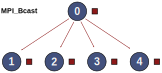
\includegraphics[width=.6\textwidth]{mpi-broadcast.pdf}%
				\fonte{Adapted from \citeonline{url:mpitutorial}.}%
			\end{figure}

		% \subsection{Scatter}

		% 	\begin{figure}[!tb]
		% 		\centering%
		% 		\caption{Example of \mpi Scatter}%
		% 		\label{fig:mpi-scatter}%
		% 		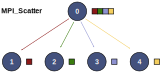
\includegraphics[width=.6\textwidth]{mpi-scatter.pdf}%
		% 		\fonte{Adapted from \citeonline{url:mpitutorial}.}%
		% 	\end{figure}

		% 	Resultados iguais ao do broadcast

		\subsection{Gather}

			% Gather é a operação inversa de uma variante do broadcast, chamada scatter. A Figura (gather) ilustra o fluxo inverso de dados, onde esta rotina reúne os  dados distribuídos em um único nó~\cite{url:mpitutorial}. De forma análoga ao broadcast, foi implementado uma flat tree onde todos os nós raízes enviam suas partes diretamente ao nó raiz.
			Gather is the inverse operation of a broadcast variant called scatter.
			\autoref{fig:exp-gather} illustrates the reverse data flow, where this
			routine gathers the data distributed on a single node~\cite{url:mpitutorial}.
			Similarly to broadcast, a flat tree was implemented where all root
			nodes send their parts directly to the root node.

			\begin{figure}[!tb]
				\centering%
				\caption{Example of \mpi Gather}%
				\label{fig:exp-gather}%
				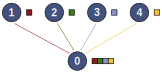
\includegraphics[width=.6\textwidth]{mpi-gather.pdf}%
				\fonte{Adapted from \citeonline{url:mpitutorial}.}%
			\end{figure}

		\subsection{AllGather}

			% AllGather é uma rotina que não possui um nó raíz, ilustrado pela Figura (allgather). Como o nome sugere, a rotina executa diversas operações Gather para que todos os nós participantes terminem com todas as partes dos dados reúnidos. Alguns algorítmos possíveis são Ring Algorithm, Recursive Doubling, Gather followed by Broadcast Algorithm. O benchmark implementa o Bruck Algorithm onde cada nó enviará seu dado para um nó com distância i e receberá dados de uma distância -i, até que todos os nós contenham o dado completo.
			AllGather is a routine that does not have a root node, illustrated by
			\autoref{fig:exp-allgather}. As the name suggests, the routine performs
			several Gather operations so that all participating nodes end with all
			pieces of data gathered. Some possible algorithms are Ring Algorithm,
			Recursive Doubling, Gather followed by Broadcast Algorithm. The benchmark
			implements the Bruck Algorithm where each node will send its data to a node
			with distance $i$ and receive data from a distance $-i$ until all nodes
			contain the complete data.

			\begin{figure}[!tb]
				\centering%
				\caption{Example of \mpi AllGather}%
				\label{fig:exp-allgather}%
				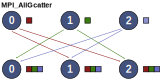
\includegraphics[width=.6\textwidth]{mpi-allgather.pdf}%
				\fonte{Adapted from \citeonline{url:mpitutorial}.}%
			\end{figure}

		\subsection{Ping-Pong}

			% Ping-pong não é uma rotina de comunicação coletiva do MPI mas representa a comunicação de um servidor respondendo requisições de nós clientes. A Figura (ping-pong) ilustra a comunicação se concentrando no nó mestre, onde o mestre recebe e responde uma requisição de cada vez.
			Ping-Pong is not an \mpi collective communication routine but represents
			communication from a server answering requests from client nodes.
			Ping-Pong illustrates communication by focusing on the master node,
			where the master receives and answers one request at a time.

			\begin{figure}[!tb]
			    \centering%
			    \caption{Example of Ping-Pong}%
			    \label{fig:exp-ping-pong}%
			    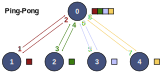
\includegraphics[width=.6\textwidth]{mpi-ping-pong.pdf}%
			    \fonte{Develop by the Author.}%
			\end{figure}

	\section{Portal Throughput Analysis}

		% O primeiro experimento buscou analiser a taxa de transferência provida pelo serviço Portal. Todos os micro-benchmarks envolvem 1 Cluster I/O e 16 Cluster de computação. A Figura (portal) mostra a taxa de transferência em megabytes por segundo, variando o tamanho do buffer a ser transmitido de 4 KB até 64 KB. Não foram testados com valores maiores que 64 KB por causa da limitação de memória nos Cluster de Computação, onde além de dividí-lo com o kernel do Nanvix, é necessário alocar tamanho suficiente para receber os dados. Por exemplo, o AllGather requer um espaço total de 1.088 MB ($17 clusters \times 64 KB$).

		% Pode-se perceber 3 comportamentos distintos nos resultados do Portal. Primeiramente, já era esperado do broadcast apresentar a pior taxa de transmissão devido ao uso de um único emissor de dados. Como a medição foi feita do lado do receptor, o último escravo teve que aguardar a transmissão para todos os outros, diminuindo consideravelmente a taxa de transferência no broadcast. Segundo, as rotinas Gather e Ping-Pong apresentaram resultados similares. Essa similaridade se deve ao fato do nó mestre receber múltiplas requisições e tratá-las de forma serial, uma a uma. Como a transferência através do Portal só é realizada quando permitida pelo receptor, o nó mestre ditou o fluxo de dados em ambos os benchmarks. Por último, a rotina AllGather apresentou os melhores resultados por causa do paralelismo das comunicações. Cada par de comunicações ocorria simultaneamente e não ocorria o caso de múltiplas leituras/escritas serem solicitadas ao mesmo tempo, amenizando a interrupção do core mestre. De forma geral, os resultados foram dentro do esperado, porém, acredita-se que o uso dos aceleradores da DMA possam melhorar bastante a performance do Portal.

		The first experiment sought to analyze the throughput provided by the
		Portal service. All micro-benchmarks involve 1 \iocluster and 16 \ccluters.
		\autoref{fig:exp-portal} shows the transfer rate in MB/s, varying the size
		of the buffer to be transmitted from 4~KB to 64~KB. They have not been
		tested with values ​​larger because of the memory limitation in the \ccluters.
		For instance, AllGather requires approximately a total space of 1~MB ($17 nodes \times 64 KB$).

		Results exhibit three distinct behaviors in the Portal results. First,
		the Broadcast was expected to have the worst transmission rate due to
		the use of a single data transmitter. Since the measurement was done
		on the receiver side, the last slave had to wait for master transmits
		to all other nodes, considerably reducing the transfer rate in the
		Broadcast. Second, the Gather and Ping-Pong routines showed similar
		results. This similarity is because the master node receives multiple
		requests and handles them serially one by one. The master node
		dictated the data flow in both benchmarks because transfer through
		the Portal is only performed when allowed by the receiver. Finally,
		the AllGather routine exhibited the best results because of the
		parallelism of communications. Also, each communication pair co-occur,
		and multiple read/write requests not happen int the same time on a node,
		softening the interruption of the master core. Overall, the results
		were as expected, but we believe that the use of \dma accelerators could
		significantly improve Portal performance.

		\begin{figure}[!tb]
			\centering%
			\caption{Throughput of the Portal.}%
			\label{fig:exp-portal}%
			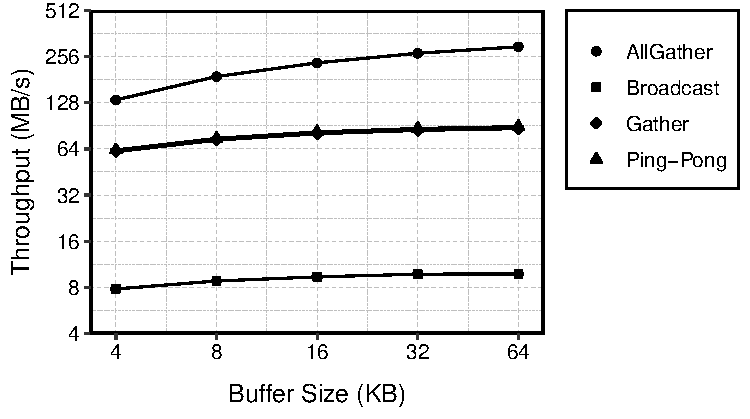
\includegraphics[width=.6\textwidth]{portal-throughput.pdf}%
			\fonte{Develop by the Author.}%
		\end{figure}

	\section{Mailbox Latency Analysis}

		% O segundo experimento teve como objetivo analisar a latência do serviço Mailbox. Os micro-benchmarks executados foram praticamente iguais, entretanto, o tamanho do buffer a ser transmitido se tornou constante, 120 Bytes. O parâmetro variável dos experimentos foi o número de Clusters de Computação envolvidos nas rotinas. Deste modo, o Cluster I/O é sempre o mestre das rotinas e altera-se a quantidade de Clusters de Computação entre 1 e 16. No caso do AllGather, o Cluster I/O também participa das comunicações.

		% De forma geral, as rotinas apresentados os comportamentos esperados. O Gather, uma das rotinas mais importantes, apresentou o melhor resultados porque o recebimento das N mensagens ocorrem paralelamente. Com isto, o custo posterior à primeira mensagem é o overhead do serviço em si, e não da comunicação. O AllGather apresentou um comportamento similar ao do Gather porque todos os cluster enviar suas mensagens antes de começarem a ler. Logo o aumento na latência é impactado pela tarefa de envio. A rotina broadcast também sofre do mesmo mal da serviço Portal, onde o fato de existir apenas um nó emitindo as mensagens impacta na latência da Mailbox. Por último, o comportamento linear da rotina Ping-Pong é cauda pelo overhead do envio das mensagens ao requisitantes. É possível notar que o Ping-Pong pode ser equiparado a soma dos custos das rotinas Gather e Broadcast, onde apesar dos benefícios do recebimento em paralelo das requisições, o mestre gasta a maior parte do tempo tratando as requisições sequencialmente.

		The second experiment aimed to analyze the latency of the Mailbox
		service. The micro-benchmarks executed were practically the same
		as the Portal. However, the buffer size to be transmitted became
		constant, 120~Bytes. The variable parameter of the experiments was
		the number of computation clusters involved in the routines.
		Thus, \iocluster is always the master of routines, and the number
		of \ccluster is changed between 1 and 16. In the case of AllGather,
		\iocluster also participates in communications.

		\autoref{fig:exp-mailbox} presents the results of the experiments.
		Generally speaking, the routines presented the expected behaviors.
		First, Gather routine, one of the essential routines, had the best
		results because receiving the messages occurs in parallel. Thus,
		the cost after the first message is the overhead of the service
		itself, not the communication. Second, AllGather routine exhibited
		similar behavior to Gather because all clusters send their messages
		before they start reading. Therefore the increase in latency is
		impacted by the transfer operation. The Broadcast routine also
		suffers from the same evil as the on Portal benchmark, where because
		exists only one node sending the messages impacts Mailbox latency.
		Finally, the linear behavior of the Ping-Pong routine is tailored
		by the overhead of sending messages to requesters. It can be noted
		that Ping-Pong can be equated to the sum of Gather and Broadcast
		costs, where despite the benefits of receiving requests in parallel,
		the master spends most of his time handling requests sequentially.

		\begin{figure}[!tb]
			\centering%
			\caption{Latency of the Mailbox.}%
			\label{fig:exp-mailbox}%
			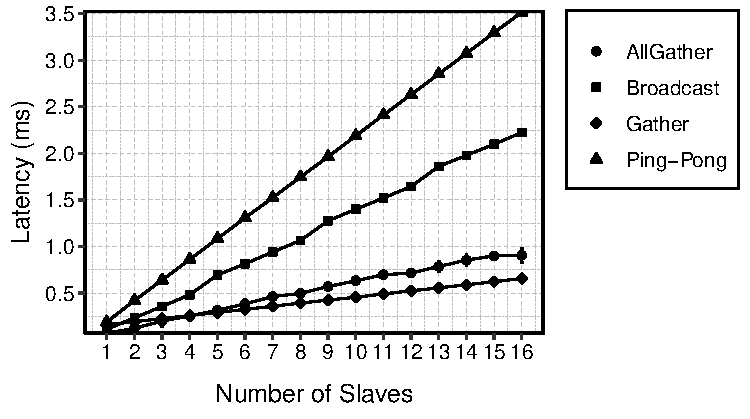
\includegraphics[width=.6\textwidth]{mailbox-latency.pdf}%
			\fonte{Develop by the Author.}%
		\end{figure}
